\documentclass[11pt]{article}

\usepackage[paper=a4paper,margin=0.75in]{geometry}
\usepackage{setspace}
\usepackage{amsmath, graphicx}
\usepackage{amsfonts,amssymb,amsthm, amsmath}
\usepackage[bottom]{footmisc}
\usepackage{mathrsfs}
\usepackage{hyperref}
\usepackage{bm}
{
        \newtheorem{assumption}{\textit{Assumption}}
        \newtheorem{definition}{\textit{Definition}}
        \newtheorem{theorem}{\textit{Theorem}}
}
\numberwithin{equation}{section}

\usepackage{fancyhdr}
\pagestyle{fancy}
\rhead{\today}
\lhead{Industrial Organisation Revision -- Lecture 2}

\newcommand\blfootnote[1]{%
	\begingroup
	\renewcommand\thefootnote{}\footnote{#1}%
	\addtocounter{footnote}{-1}%
	\endgroup
}

\begin{document}

\section{Market Power in Differentiated Goods Markets}\label{s1}
\blfootnote{These notes are based on Howard Smith's lectures from the 2018-2019 academic year.\\
Of course, this is our interpretation of the material Howard presented. Good content is his; mistakes are ours.}

\vspace{-1cm}
\begin{itemize}
	\item Basic problem: Want to estimate a $J\times 1$ demand system $q=q(p,\theta)$ defined in $J$ prices. We initially (in this section) attempt to do this in the most general way possible.
	\item For item/firm $j$ we have
	\begin{itemize}
		\item demand $q_j(p,\theta)$, and
		\item profit $q_j(p,\theta)(p_j - mc_j)$.
	\end{itemize}
	\item Profit $\pi_f$ for firm $f$ with products $k\in \mathscr{F}_f$ is $\pi_f \equiv \sum_{k\in \mathscr{F}_f}q_k(p,\theta)(p_k - mc_k)$.
	\item Firm $f$'s profit maximizing condition for price $j$ assuming multiproduct Nash behaviour\footnote{i.e. prices being set conditioning on other firms' prices and internalising cross-product effects.} is
	\begin{equation}\label{s1.eq1}
	 \frac{\partial \pi_f}{\partial p_j} = \sum_{k\in \mathscr{F}_f} \frac{\partial q_k(p,\theta)}{\partial p_j}(p_k - mc_k) + q_j(p,\theta) = 0.
	\end{equation}
	Equation \ref{s1.eq1} encapsulates the \emph{two} sources of market power in this model:
	\begin{itemize}
		\item \emph{product differentiation}: corresponds to element $\frac{\partial q_j(p,\theta)}{\partial p_j}$, present in both single- and multiproduct environment, and;
		\item \emph{portfolio effect}: corresponding to elements of the sort $\frac{\partial q_k(p,\theta)}{\partial p_j}$, $\forall k\neq j$; present only for multi-product firms.
	\end{itemize}
	\item Define  $\Delta(p,\theta)$ to be a $J\times J$ block-diagonal matrix with zero off-diagonal blocks. Blocks along the diagonal are square matrices, with $card(\mathscr{F}_f)^2$ elements; the number of blocks is equal to the number of firms, and the block indexed by $f$ contains $\frac{\partial q_k(p,\theta)}{\partial p_j}$, $\forall j,k\in \mathscr{F}_f$, with $k$ indexing rows and $j$ indexing columns. Now we can write
	\begin{equation}
		\Delta(p,\theta)[p - mc] + q(p,\theta) = 0
	\end{equation}
	for the system of $J$ optimality conditions, yielding
	\begin{equation}
		p =  mc - [\Delta(p,\theta)]^{-1} q(p,\theta).
	\end{equation}
	%This is one bad mother-fucker.
	The term $[\Delta(p,\theta)]^{-1} q(p,\theta)$ encapsulates both sources of market power in the multiproduct Nash model.
	\item If we could get data on or estimate $mc$ and estimate $\theta$, then (with functional form assumptions) we can estimate the effect of mergers/demergers by changing elements in $\Delta(p,\theta)$. E.g. under monopoly there are no zero blocks in $\Delta(p,\theta)$ -- i.e. portfolio effects are non-zero as the monopolist accounts for all price effects in her profit maximisation; in case of a demerger across all products, $\Delta(p,\theta)$ becomes diagonal and portfolio effects disappear (still left with distortion from product differentiation).
	\item Important example: collusion. To incorporate collusion, all we need to do is alter $\Delta(p,\theta)$ so that some share of other firms' profit enters profit for each firm $f$. Denote this by $\Delta(p,\theta,\kappa)$, assuming that share is a constant $\kappa$ across all firms. Now the block-off-diagonals for the rows belonging to block $f$ in $\Delta(p,\theta,\kappa)$ correspond to $\kappa\frac{\partial q_{k'}(p,\theta)}{\partial p_j}$ for $k'\notin \mathscr{F}_f$ and $j\in \mathscr{F}_f$, and our optimality conditions are
	\begin{equation}
	p =  mc - [\Delta(p,\theta, \kappa)]^{-1} q(p,\theta).
	\end{equation}
	\item In this last example, if we assume $mc$ is constant across products, we have $J(1+J)$ parameters to estimate. We can attempt to estimate such a model with market-level data $\{s_{jt}, p_{jt}, x_{jt}\}$, where $s_{jt}$, $p_{jt}$ and $x_{jt}$ are market shares (quantity), prices and product characteristics respectively, with $j=1,\dots,J$ and $t=1,\dots,T$. Could also user consumer-level data.
\end{itemize}

\section{Estimating $\theta$ via discrete choice models (Demand Side)}
\subsection{Logit}

\begin{itemize}
	\item Let $\theta = (\beta, \alpha)$. Consumer $i$'s utility for product $j\in \mathscr{F} =\{0,\dots,J\}$ is:
	\begin{equation}
		u_j^i = \beta x_j - \alpha p_j + \xi_j + \epsilon_j^i \equiv \delta_j + \epsilon_j^i
	\end{equation}
	\begin{itemize}
		\item[-] $\beta$: vector of marginal valuations of characteristics $x_j$ (these are common utility function parameters)
		\item[-] $\alpha$: price sensitivity; marginal utility of money
		\item[-] $\xi_j$: mean utility of $j$'s unobserved characteristics
		\item[-] $ \delta_j \equiv \beta x_j - \alpha p_j + \xi_j $: mean utility of product $j$ (common across consumers -- note, assumes $\epsilon_j^i$ are mean zero, but not true for Type 1 Extreme Value).
		\item[-] $\epsilon_j^i$ is consumer $i$'s individual unobserved utility from product $j$.
	\end{itemize}
	\item $i$ chooses $j \iff (u_i^j \geq u_i^k\quad \forall k \in \mathscr{F})$ where $\mathscr{F}$ is the choice set.
	\item Type-1 extreme value (EV(0,1)):
	\begin{itemize}
		\item $F(\epsilon)=\text{exp}(-\text{exp}(-\epsilon));\, f(\epsilon)=\text{exp}(-\epsilon)\text{exp}(-\text{exp}(-\epsilon))$; with support $\Re^n$.
		\item $\text{Pr}(u_i^j \geq u_i^k\quad \forall k \in \mathscr{F}) = \frac{e^{\delta_j}}{\sum_{k=0}^{J}e^{\delta_k}} = \frac{e^{\delta_j}}{1 + \sum_{k=1}^{J}e^{\delta_k}}$; ($\delta_0=0$ by normalization).\footnote{See Appendix \ref{logitderiv}.}
		\item First order statistic (expected maximum value) of $u_j^i$ for $j$ in $\mathscr{F}'\subset\mathscr{F}$:
		\begin{equation}
			CS = \frac{1}{\alpha}\mathbb{E}\bigg[\max_{j\in \mathscr{F}'}(\delta_j + \epsilon_j^i)\bigg] = \frac{1}{\alpha}\log{\bigg[\sum_{j\in \mathscr{F}'}\text{exp}(\delta_j)]\bigg]}
		\end{equation}
		\item When $\mathscr{F}'=\mathscr{F}$, $CS$ is a measure of consumer surplus of the choice set (the ``log sum'' or ``inclusive value'').
		\item Yields linear model:
		\begin{equation}
			s_j = \frac{e^{\delta_j}}{\sum_{k=0}^{J}e^{\delta_k}} \implies \log{s_j} = \delta_j - \log{\sum_{k=0}^{J}e^{\delta_k}}
		\end{equation}
		and thus
		\begin{equation}
			\log{s_j} - \log{s_0} = \delta_j = \beta{}x_j -\alpha{}p_j + \xi_j
		\end{equation}
		which can be used to estimate $\theta = (\beta, \alpha)$ with $\xi_j$ treated as a residual and $j=1,\dots,J$ indexing observations.
	\end{itemize}
	\item For OLS, must assume $\mathbb{E}[\xi_j|(x_j,p_j)]=0$; $\xi$ observed by seller (possibly by buyer too) so unlikely to hold.
  IV estimation requires $\mathbb{E}[\xi_j|(x_j,z_j)]=0$ for some $z_j$ (instrument validity).
  Candidate $z_j$'s: Marginal cost shifters; product characteristics not in utility; prices of the same product in other cities (Hausman).
  Might also want instruments for non-price characteristics $x_j$.
	\item Logit elasticities:
	\begin{itemize}
		\item $\frac{\partial s_j}{\partial p_j} = -\alpha s_j(1-s_j) \implies \frac{\partial s_j}{\partial p_j}\frac{p_j}{s_j} =  -\alpha p_j(1-s_j)$
		\item $\frac{\partial s_k}{\partial p_j} = -\alpha s_js_k \implies \frac{\partial s_k}{\partial p_j}\frac{p_j}{s_k} = -\alpha s_j p_j \quad \forall k\neq j$, which is \emph{independent of $k$}.
		\item Very inflexible; no effect from closeness of the two products observed characteristics.
	\end{itemize}
\end{itemize}

\subsection{(Random Coefficients) Mixed Logit}
\begin{itemize}
	\item Used by Berry, Levinsohn and Pakes (1995); $\beta$'s now vary across consumers:
	\begin{equation}
		u_j^i = \beta^ix_j - \alpha p_j + \xi_j + \epsilon_j
	\end{equation}
	with
	\begin{equation}
		\beta_a^i = \bar{\beta}_a + \sigma_a\nu_a^i
	\end{equation}
	\begin{itemize}
		\item $\bar{\beta}_a$, mean value of characteristic $a$.
		\item $\nu_a^i \sim F(\nu)$, individual $i$'s taste for $a$ relative to mean taste; distributed $F(\nu)$, density $f(\nu)$.
		\item $\sigma_a$, scaling term; spread of taste variation of $a$.
	\end{itemize}
	\item Realised utility is then given as
	\begin{flalign}
	u_j^i & = \sum_{a}[\bar{\beta} + \sigma_a\nu_a^i]x_{ja} - \alpha p_j + \xi_j + \epsilon_j^i \\
	& \equiv \delta_j + \sum_{a} \sigma_a\nu_a^ix_{ja} + \epsilon_j^i.
	\end{flalign}
	with $\delta_j \equiv \bar{\beta}x_j - \alpha p_j + \xi_j$ (i.e. product characteristics).
	\item Conditioning on $i$'s draw of $\nu^i$ we have standard closed form for the individual's choice probability:
	\begin{equation}
    \label{rcml_ratio}
		\text{Pr}(u_j^i > u_l^i ~\forall~ k\neq l~|~\nu^i) = \frac{\text{exp}(\delta_j + \sum_{a}\sigma_a\nu_a^i x_{ja})}{1 + \sum_{k=1}^{J}\text{exp}(\delta_k + \sigma_a\nu_a^i x_{ka})}
	\end{equation}
	i.e.\ we have logit conditional on the $\nu^i$'s; $\sigma_a$ adds flexibility/heterogeneity in preferences for $x$; this means that person with taste for specific characteristics will substitute more readily to alternatives with similar characteristics.
	\item Obtaining $s_j$:
	\begin{itemize}
		\item Integrate over density $f(\nu)$ in the population of consumers:
		\begin{equation}
		s_j(\xi,\theta) \overset{\eqref{rcml_ratio}}{=} \int_{v}\left(\frac{\text{exp}(\delta_j + \sum_{a}\sigma_a\nu_a^i x_{ja})}{1 + \sum_{k=1}^{J}\text{exp}(\delta_k + \sigma_a\nu_a^i x_{ka})}\right) f(\nu)d\nu
		\end{equation}
		\item 	We do not know $\theta = (\beta, \alpha, \sigma)$ or $\xi$, and there is no analytic form for this integral, but for a given $(\xi, \theta)$ we can evaluate the integral via numerical (Monte Carlo) integration: assuming a density $f(\nu)$ for $\nu$, draw $ns$ values of $\nu^i$ from $f(\nu)$ and compute
		\begin{equation}\label{eqn.marketshare}
		s_j(\xi,\theta)^{sim} = \frac{1}{ns} \sum_{i=1}^{ns}\frac{\text{exp}(\delta_j + \sum_{a}\sigma_a\nu_a^i x_{ja})}{1 + \sum_{k=1}^{J}\text{exp}(\delta_k + \sigma_a\nu_a^i x_{ka})}
		\end{equation}
	\end{itemize}
	\item Estimation:
	\begin{enumerate}
		\item Assume that at true $\theta = (\alpha, \beta, \sigma)$ the unobserved utility $\xi$ is mean-independent of product characteristics $x$ and other instruments $z$, i.e. $\mathbb{E}[\xi(\theta)|x,z]=0$, and estimate using these moment conditions in a GMM estimator.
		\item For observations $(\hat{p}, \hat{x}, \hat{s})$ and trial parameter values $\theta_t$ there is a unique $J$-vector $\xi$ implied by inverting the market share equation \ref{eqn.marketshare}: $\hat{s} = s^{sim}(\xi, \theta_t) \implies \xi = \xi(\theta_t,\hat{s})$.
    This inversion is possible because the market share function is one-to-one: for each $j$, $\hat{s}$ is a smooth function monotonically increasing in $\xi_j$ and decreasing in $\xi_k$ for all $k\neq j$ (Berry, 1994 conditions).
		\item No closed form solution for $\xi = \xi(\theta_t,\hat{s})$; must be solved numerically at each trial $\theta_t$. This is achieved via the contraction mapping:
		\begin{equation}
		\xi_n = \xi_{n-1} + \text{ln}\bm{s} - \text{ln}\bm{s}^{sim}(\xi_{n-1},\theta)
		\end{equation}
		until some level of tolerance is achieved.
	\end{enumerate}
\end{itemize}

\section{Ackerberg, Benkard, Berry, and Pakes (2007, Section 1)}
\subsection{Demand Side Model}
	\begin{itemize}
	\item Let individual $i$'s utility from product $j$ at time/in market $t$\footnote{$t$ dropped in the following for simplicity.} be $u_{ijt} = U(\tilde{x}_{jt}, \xi_{jt}, z_{it}, \nu_{it}, y_{it} - p_{jt}, \theta)$ where:
	\begin{itemize}
		\item $\tilde{x}_{jt}$ is a $K$-dimensional vector of observed product characteristics other than price;
		\item $p_{jt}$ is the price of the product;
		\item $\xi_{jt}$ are the unobserved characteristics of the product (allowed to vary over $t$);
		\item $z_{it}$ and $\nu_{it}$ are differences in taste of consumer $i$, respectively observed and unobserved by the econometrician;
		\item $y_{it}$ is consumer $i$'s income;
		\item $\theta$ is the vector of parameters to be estimates.
	\end{itemize}
	\item The partial equilibrium nature of the problem is incorporated into the model
	by letting utility depend on the money available to spend outside of this market ($y_{i} - p_{j}$) (quasi-linear preferences assumed implicitly); sometimes expenditure in other markets is not ``explicitly'' modelled (as it is here). Then utility is of the form $u_{ij} = U(\tilde{x}_{j}, \xi_{j}, z_{i}, \nu_{i}, p_{j}, \theta)$; this is the form they seem to actually work with.
	\item The model incorporates an option ``purchase nothing'' as the outside good $j=0$ with utility $u_{i0} = U(\tilde{x}_{0}, \xi_{0}, z_{i}, \nu_{i}, \theta)$.
	\item Product choice is determined by $u_{ij}>u_{ir},~\forall~ r \neq j$.
	\item Assuming linearity and letting $x_j := (\tilde{x}_j, p_j)$ we have $U_{ij} = \sum_{k}x_{jk}\theta_{ik} + \xi_j + \epsilon_{ij}$, with $\theta_{ik} = \bar{\theta}_k + \theta_j^o\prime z_i + \theta_j^u\prime \nu_i$; i.e. the observed and unobserved taste parameters interact with the product characteristics. $U_{i0}=0$ by normalization.
	\item Unobserved product characteristics $\xi_j$ \textbf{must be characterisable as a scalar}; taste for this characteristic is assumed not to vary across consumers (this is a real assumption -- not a normalisation -- that implies $\xi_j$ can be thought of as a residual).
	\item $\epsilon_{ij}$'s are a bit awkward; taste variation for product $j$ of individual $i$ that is independent across products and individuals. Can do away with this term; leads to model with nice properties, but it is computationally convenient to keep $\epsilon_{ij}$'s.
	\item Substituting in the expression for $\theta_{ik}$ (remember, $i,k$ is an individual-characteristic pair) we obtain
	\begin{equation}\label{eqn.paper6}
	U_{ij} = \delta_j + \sum_{kr}\theta_{rk}^u x_{jk} z_{ir} + \sum_{kl}\theta_{lk}^u x_{jk} \nu_{il} + \epsilon_{ij}
	\end{equation}
	where $r$ and $l$ index the elements in $z_{i}$ and $\nu_i$ respectively, and
	\begin{equation}
	\delta_j = \sum_{k}\bar{\theta}_kx_{jk} + \xi_j.
	\end{equation}
	\item The interactions of $x_{jk}$ with $z_{i}$ and $\nu_{i}$ are what generate flexible own and cross price elasticities.
	\end{itemize}

\subsection{Estimation with Product-Level Data}
	\begin{itemize}
		\item With product level data, $z_i\equiv 0$ for all $i$ (no individuals are observed). For elements in $\nu_i$ we might have some data sources (e.g. census data) yielding the relevant distribution; if we don't, we assume some parametric distribution for $\nu_i$ (preferably one we can draw from) and include the parameters of that distribution in our vector of parameters we wish to estimate -- for example, we might assume a normal distribution for $\nu_i$ with mean and standard deviation vectors $\bar{\theta}$ and $\theta^u$ respectively.

		\item Since $\xi_{j}$'s are likely correlated with elements in $x_{j}$, we require a set of instruments $w_{j}$ such that $\mathbb{E}(\xi_j | w_j)=0$.\footnote{Is this maybe a stronger assumption than necessary? Could we merely have assumed orthogonality?}
		\item Steps in estimation are actually quite simple:
		\begin{enumerate}
			\item Get an estimate of $\xi(\cdot)$ as a function of $\theta$ -- i.e. we need an estimate of a function that varies in the parameters of the model; this is really conceptually the same as OLS, wherein the errors are also functions of the model parameters;
			\item Make some identifying assumptions on $\xi(\cdot;\theta)$, specifying that at the true value of the parameters ($\theta=\theta_0$) it obeys some restrictions -- this is where we use our instruments;
			\item Use a standard method of moments estimator to impose the identifying restrictions and back out the unique value of $\theta$ such that $\xi(\cdot;\theta)$ satisfies our restrictions.
		\end{enumerate}
		\item Step I: Evaluate, for candidate parameter vector, the integral
		\begin{equation}
		\sigma_j(\delta,\theta) = \int_{v}\left(\frac{\text{exp}(\delta_j + \sum_{kl}x_{jk}\nu_{lr}\theta_{kl}^u)}{1 + \sum_{q=1}^{J}\text{exp}(\delta_j + \sum_{kl}x_{jq}\nu_{lr}\theta_{ql}^u)}\right) f(\nu)d\nu.
		\end{equation}
		numerically as
		\begin{equation}
		\sigma_j(\delta,\theta,P^{ns}) = \sum_{r=1}^{ns}\frac{\text{exp}(\delta_j + \sum_{kl}x_{jk}\nu_{lr}\theta_{kl}^u)}{1 + \sum_{q=1}^{J}\text{exp}(\delta_q + \sum_{kl}x_{jq}\nu_{lr}\theta_{ql}^u)}.
		\end{equation}
		The key thing to note here is that once you have your draws of $\nu_{lr}$ (i.e. you have $P^{ns}$, the empirical distribution of your simulation draws) you can evaluate this thing at different values of $\xi,\theta$.
		\item Step II: From the empirical market shares $s^n = [s^n_1,\dots, s^n_J]$, where $n$ denotes the size of the sample from which these shares are calculated (often large -- but if we have market level data we don't have this sample), find the unique vector $\delta$ that makes the predicted shares $\sigma_j(\xi,\theta,P^{ns})$ equal the actual shares $s^n$ for a given value of $\theta$ and simulation draws $P^{ns}$. This is achieved via the contraction mapping (as shown by BLP 1995):
		\begin{equation}
		\delta_j^k(\theta) = \delta_j^{k-1} + ln[s^n]-ln[\sigma_j(\delta_j^{k-1},\theta,P^{ns})].
		\end{equation}
		where $k$ indexes loop iterations. Recall that $\delta$ is a function of some elements in $\theta$; but of course we're not allowing theta to vary here -- only $\delta$, and by implication $\sigma_j(\delta_j^{k-1},\theta,P^{ns})$ is changing. We stop this process when $\sigma_j(\delta_j^{k-1},\theta,P^{ns})$ and $s_j^n$ are ``close enough''. Call the fixed point obtained by this process $\delta(\theta,s^n,P^{ns})$. The model \ref{eqn.paper6} then implies that
		\begin{equation}
		\xi_j(\theta,s^n,P^{ns}) = \delta(\theta,s^n,P^{ns}) - \sum_{k}x_{jk}\bar{\theta}_k.
		\end{equation}
		I.e. we've managed to obtain an estimate of the $\xi_j$'s as a function of the model parameters $\theta$; this thing varies as we vary $\theta$, so now we need to specify the restrictions on $\xi_j$ and vary $\theta$ until we find the set of parameters that most closely satisfies those restrictions.

		Side note on \emph{identification}: As mentioned, identification here follows from restrictions on the true distribution of $\xi$; for identification, as $n$ and $ns$ go to infinity, $\xi(\theta,s^{\infty},P^{\infty})$ will/must uniquely satisfy these restrictions at $\theta=\theta_0$. You could use different restrictions to achieve this result; we work with $\mathbb{E}[\xi(\theta_0)|w]=0$, which leads to the third and final step of the algorithm:
		\item Step III: Minimize $||G_{j,n,ns}(\theta)||$ over $\theta$, where
		\begin{equation}
		G_{j,n,ns}(\theta) = \sum_{j}^{J}\xi(\theta,s^{n},P^{ns})f(w_j).
		\end{equation}
		Note that given $\theta^u$ there is a closed form solution for $\bar{\theta}$; so the nonlinear search is over $\theta^u$ only.
	\end{itemize}

\subsection{Improving Efficiency}
	\begin{itemize}
		\item ABBP (2007) also discuss improving model efficiency via jointly estimating the pricing equation outlined in section \ref{s1};
		\item requires assumptions regarding the functional form of the marginal cost function, as well as assumptions on the market structure (as outlined above).
		\item Alternatively, micro data can be used to improve efficiency.
		\item Especially useful when second choice data or panel data are available, but details on individual characteristics also useful (allows us to shift some elements out of $\nu$ and into $z$).
		\item If we don't have data on individual choice behaviour, we can still use micro data to draw values of $\nu$ for simulating the model with market level data.
		\item Almost nothing changes when we have micro data on consumers -- all we need do is distinguish between the observed and unobserved taste shifters in the market share equation:
		\begin{equation}
		\sigma_j(\delta,\theta) = \int_{v}\left(\frac{\text{exp}(\delta_j + \sum_{kl}x_{jk}z_{lr}\theta_{kl}^o + \sum_{kl}x_{jk}\nu_{lr}\theta_{kl}^u)}{1 + \sum_{q=1}^{J}\text{exp}(\delta_q  + \sum_{kl}x_{jk}z_{lr}\theta_{kl}^o+ \sum_{kl}x_{jq}\nu_{lr}\theta_{ql}^u)}\right) f(\nu)d\nu.
\end{equation}
\end{itemize}

\section{Application: Miller and Weinberg (2017)}

The authors estimate a differentiated-goods pricing model with a random coefficients mixed logit demand side to explore the implications of the Miller-Coors joint venture for the beer market.
Analysis based on market level data from 2001-2010 for multiple bundles of beer and multiple producers. \\

The basic idea is that the merger could have moved the market to a new equilibrium with facilitated price coordination with ABI, a large competitor.
The table below shows that the post-merger price changes for Miller-Coors and ABI are impressively close regardless of specification, which in principle is consistent with the idea of a coordination equilibrium.

\begin{center}
	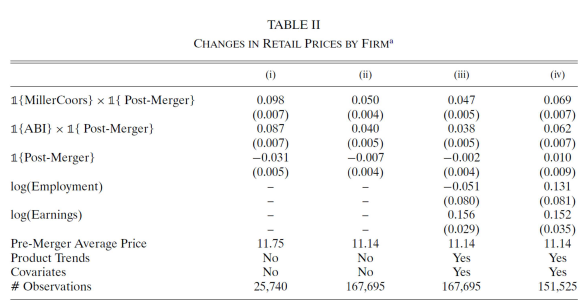
\includegraphics[width=0.7\textwidth]{mw1}
\end{center}

The demand side is standard random coefficients mixed logit with the sole purpose of providing a way of quantifying cross-price elasticities before and after the merger.
Refer to previous sections for estimation; the only thing worth noting is that the set of instruments used include cost shifters (distance from factory) and a post-merger indicator -- under the assumption of exogeneity of the merger with respect to the competitive environment.  \\

The supply model allows for post-merger departures from Nash-Bertrand play for Miller-Coors and ABI, while forcing other competitors to play Nash-Bertrand.
The assumption that changes in post-merge unobserved demand for ABI are not different from changes for other competitors allows to \textbf{identify collusion as price response in excess} of what can be explained by unilateral effects. \\

The demand side of the model is estimated first; these estimates are then used to populate the cross-price effects matrix and estimate the supply side in search for collusion.
The demand side is \textbf{not} estimated before and after the merger: instead, the authors use estimated cross-price elasticities from the pre-merger period to populate the post-merger $\Delta(\kappa, p, \hat{\theta})$ matrix and to estimate $\kappa$ (assumed constant).
In particular, remember that for the supply side we have
\begin{equation*}
  p = mc - [\Delta(\kappa, p, \hat{\theta})]^{-1}q(p,\hat{\theta})
\end{equation*}
where $\hat{\theta}$ are demand parameters; for $mc = w\gamma + \eta$, this implies
\begin{equation}
  p = w\gamma + \eta - [\Delta(\kappa, p, \hat{\theta})]^{-1}s
\end{equation}
clearly, endogeneity of $\Delta$ prevents direct estimation of this equation; however, post-merger dummies again save the day as instruments allowing to identify $(\kappa, \gamma)$.
The table below clearly shows that \textbf{the null of no collusion is rejected}. \\

\begin{center}
	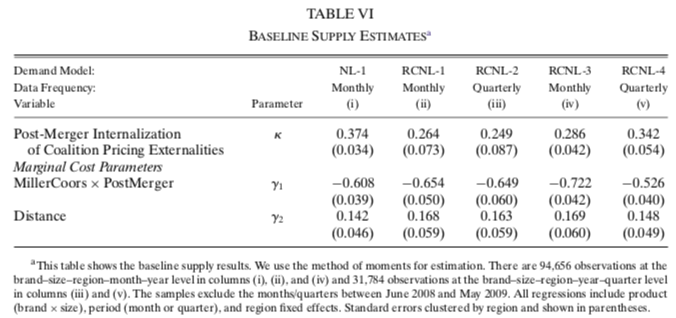
\includegraphics[width=0.7\textwidth]{mw2}
\end{center}


\begin{center}
	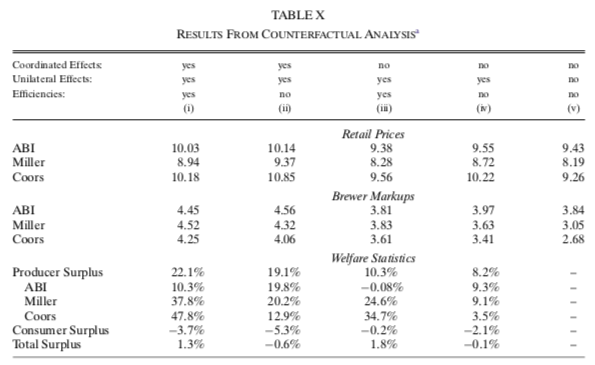
\includegraphics[width=0.7\textwidth]{mw3}
\end{center}

The counterfactual analysis exercise shows that the merger increases producer surplus by more than 20\%, with around half of these gains resulting from coordination; consumer surplus is however reduced.
In total, the merger increases welfare by around 1\%, but this increase would have been higher under no coordination.


\appendix

\section{Derivation of Logit functional form}
\label{logitderiv}
\begin{equation*}
  \begin{gathered}
  \text{Pr}(u^i_j \geq u^i_k) = \text{Pr}(\epsilon^i_k \leq \delta^i_j - \delta^i_k + \epsilon^i_j ) \Rightarrow  \text{Pr}(\epsilon^i_k \leq \delta^i_j - \delta^i_k + \epsilon^i_j  ~|~ \epsilon^i_j) = \Pi_{k \neq j} e^{e^{- (\epsilon^i_j + \delta^i_j - \delta^i_k)}} \\
  \Rightarrow \text{Pr}(\epsilon^i_k \leq \delta^i_j - \delta^i_k + \epsilon^i_j ) = \int_\epsilon (\Pi_{k \neq j} e^{-e^{- (\epsilon^i_k + \delta^i_j - \delta^i_k)}}) e^{- \epsilon^i_k}e^{-e^{- \epsilon^i_k}} d \epsilon^i_k = \int_\epsilon (\Pi_{k} e^{-e^{- (\epsilon^i_k + \delta^i_j - \delta^i_k)}}) e^{- \epsilon^i_k} d \epsilon^i_k = \\
  = \int_\epsilon e^{-\sum_{k}{e^{- (\epsilon^i_k + \delta^i_j - \delta^i_k)}}} \underbrace{e^{- \epsilon^i_k} d \epsilon^i_k}_{c.o.v. \rightarrow dt} =
  \int^\infty_0 e^{-t \sum_{k}{e^{- (\delta^i_j - \delta^i_k)}}} dt = \bigg[\frac{e^{-t \sum_{k}{e^{- (\delta^i_j - \delta^i_k)}}}}{- \sum_{k}{e^{- (\delta^i_j - \delta^i_k)}}}\bigg]^\infty_0 = 0 - \frac{1}{- \sum_{k}{e^{- (\delta^i_j - \delta^i_k)}}} = \\
  \frac{1}{\sum_{k}{e^{- (\delta^i_j - \delta^i_k)}}} = \frac{e^{\delta^i_j}} {\sum_{k}{e^{\delta^i_k}}} \qed
  \end{gathered}
\end{equation*}


\end{document}
